\chapter{The Fourier Transform and Frequency-Domain Filtering}
\label{ch:lesson15}

Every filter so far has worked directly on pixel neighborhoods. The Fourier transform offers a completely different view: any image can be rewritten as a sum of sinusoidal gratings at different frequencies and orientations. Filtering can then be done by directly boosting or suppressing specific frequencies --- and, thanks to the \textbf{convolution theorem}, this turns out to be mathematically the same operation as spatial convolution, just seen from a different angle.

\section{1D warm-up: a signal as a sum of sinusoids}

Any signal can be approximated by adding up sine and cosine waves of different frequencies. A square wave, for example, is the sum of sine waves at increasing (odd) frequencies with decreasing amplitude. The Fourier transform is the tool that goes the other way: given a signal, it tells you exactly which frequencies (and how much of each) are present, as Figure~\ref{fig:l15-1} shows by approximating a square wave.

\begin{figure}[h]
\centering
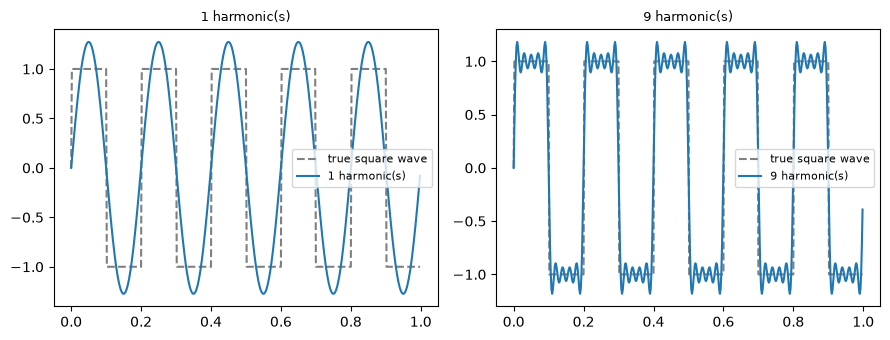
\includegraphics[width=0.75\textwidth]{figures/lesson15_fig01.png}
\caption{A square wave approximated with 1 harmonic and with 9 harmonics --- more harmonics track the true square wave more closely, especially near the sharp transitions.}
\label{fig:l15-1}
\end{figure}

\section{The 2D Fourier transform of an image}

The 2D discrete Fourier transform (DFT) of an image decomposes it into 2D sinusoidal gratings at every combination of horizontal and vertical frequency, computed via the fast Fourier transform (\code{np.fft.fft2}), which produces a complex-valued 2D array. As with the image gradient, we usually view the Fourier transform's \textbf{magnitude} (how much of each frequency is present). Two common visualization tricks, shown in Figure~\ref{fig:l15-2}: show the magnitude on a log scale, and shift the zero-frequency (average brightness) term from the top-left corner to the center.

\begin{figure}[h]
\centering
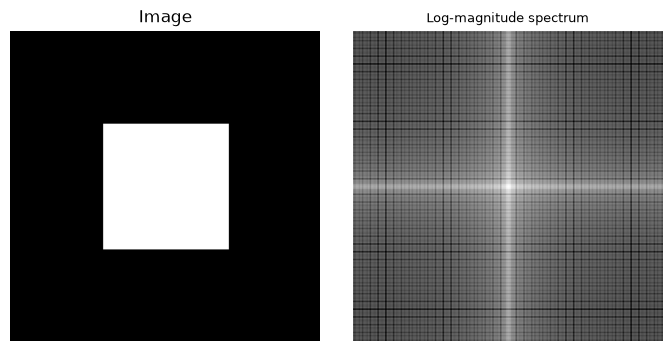
\includegraphics[width=0.65\textwidth]{figures/lesson15_fig02.png}
\caption{A filled square and its log-magnitude spectrum. The bright cross through the center comes from the square's sharp horizontal and vertical edges --- a hard step edge contains energy at \emph{every} frequency along the direction perpendicular to it, which is why a sharp-edged shape has such a spread-out spectrum.}
\label{fig:l15-2}
\end{figure}

\subsection*{A grating reveals its frequency directly as a spectrum peak}

A pure sinusoidal grating is the simplest possible test: its spectrum should be (almost) a single pair of bright dots, at a distance from the center equal to its frequency, in the direction perpendicular to its stripes.

Why a \emph{pair}, not one dot? A real-valued sine wave is, by Euler's formula, a mix of two complex exponentials in equal amounts: $\sin(2\pi fx) = \tfrac{1}{2i}(e^{i2\pi fx} - e^{-i2\pi fx})$. The Fourier transform of the first exponential is a spike at frequency $f$, and of the other at $-f$. So a real sinusoid produces two spikes at $+f$ and $-f$, symmetric about the zero-frequency (DC) center --- in fact, for \emph{any} real-valued image, its Fourier magnitude is symmetric: $|F(-f)|=|F(f)|$, as confirmed by the grating in Figure~\ref{fig:l15-3}.

\begin{figure}[h]
\centering
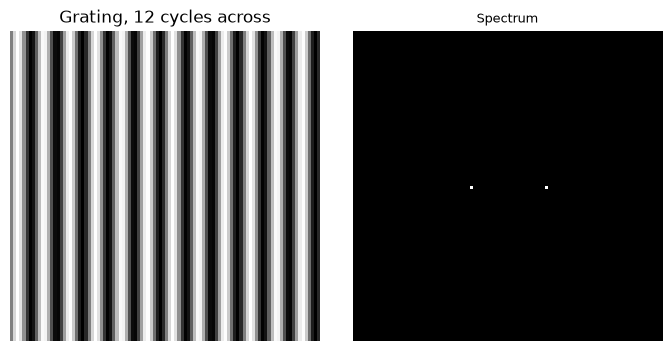
\includegraphics[width=0.6\textwidth]{figures/lesson15_fig03.png}
\caption{A grating with 12 cycles across the image and its spectrum. The brightest spectrum point lands at offset $-12$ from center, matching the grating's true frequency of 12.}
\label{fig:l15-3}
\end{figure}

\section{Filtering by editing the spectrum}

An \textbf{ideal low-pass filter} keeps only frequencies inside a circle around the center (blurs); an \textbf{ideal high-pass filter} keeps only frequencies outside it (edge-enhances). Once an image is transformed to the frequency domain, filtering is masking frequencies directly, then transforming back with the inverse transform --- since the mask is the same size as the image, this is a plain elementwise multiply.

\begin{lstlisting}
def apply_frequency_filter(image, mask):
    F = np.fft.fftshift(np.fft.fft2(image))
    filtered = np.fft.ifft2(np.fft.ifftshift(F * mask))
    return np.real(filtered)
\end{lstlisting}

Figure~\ref{fig:l15-4} shows the two masks, and Figure~\ref{fig:l15-5} the resulting filtered images.

\begin{figure}[h]
\centering
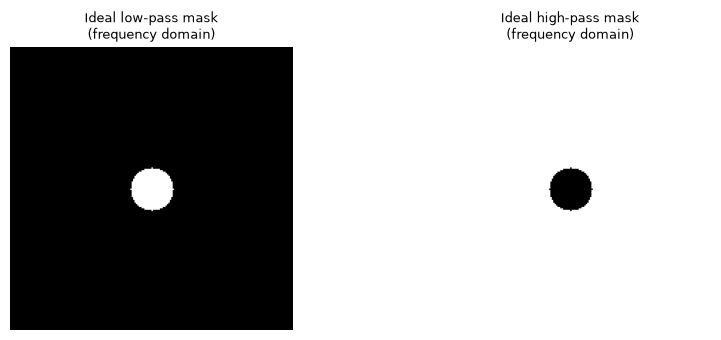
\includegraphics[width=0.85\textwidth]{figures/lesson15_fig04.png}
\caption{Ideal low-pass and high-pass masks in the frequency domain.}
\label{fig:l15-4}
\end{figure}

\begin{figure}[h]
\centering
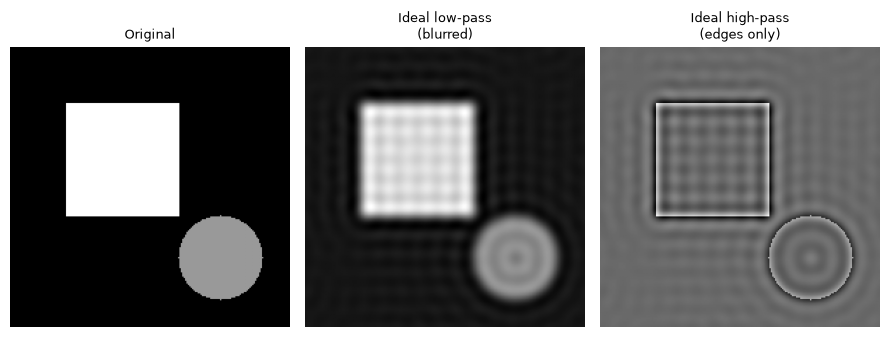
\includegraphics[width=0.9\textwidth]{figures/lesson15_fig05.png}
\caption{Original image, ideal low-pass result (blurred), and ideal high-pass result (edges only).}
\label{fig:l15-5}
\end{figure}

\subsection*{The cost of a sharp cutoff: ringing}

Faint ripples radiate from the shape edges in the ideal-filter results above. An \emph{ideal} filter has a perfectly sharp cutoff in frequency, which corresponds (by the same convolution theorem) to convolving with a spatial kernel that has infinite ripples of its own (a sinc function) --- the \textbf{Gibbs phenomenon}. A Gaussian mask, which falls off smoothly instead of cutting off sharply, avoids this, as Figure~\ref{fig:l15-6} shows.

\begin{figure}[h]
\centering
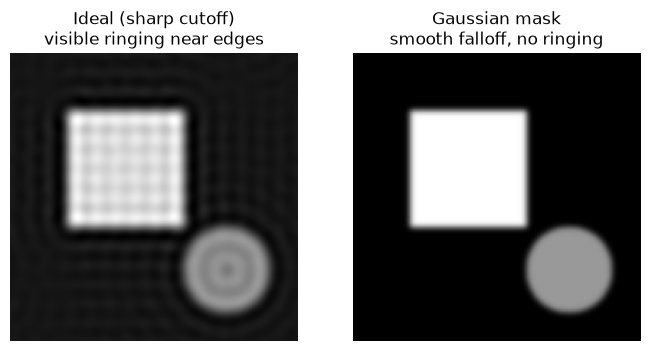
\includegraphics[width=0.65\textwidth]{figures/lesson15_fig06.png}
\caption{Ideal low-pass (sharp cutoff, visible ringing near edges) vs.\ a Gaussian mask (smooth falloff, no ringing).}
\label{fig:l15-6}
\end{figure}

\section{The convolution theorem}

Why does frequency-domain filtering work? The \textbf{convolution theorem}
\begin{equation}
\mathcal{F}\{f * g\} = \mathcal{F}\{f\} \cdot \mathcal{F}\{g\}
\end{equation}
says that convolving two signals in the spatial domain is \emph{exactly} the same as multiplying their Fourier transforms elementwise, then transforming back --- convolution becomes multiplication, and vice versa.

\subsection*{A catch: the DFT gives circular convolution}

The DFT implicitly treats the image as if it were infinitely repeating (seamless tiles extending forever in both directions) --- there is no ``outside the image,'' only ``the next copy of the same image.'' So multiplying two DFTs and transforming back doesn't give the ordinary (``linear'') convolution from Chapter~\ref{ch:lesson10}, where the kernel eventually slides off the edge into some explicit border; rather, it gives \textbf{circular convolution}, where the kernel that slides off the right edge wraps around and picks up pixels from the left edge instead. The two only agree if the border handling on the spatial side is \emph{also} wraparound (\code{cv2.BORDER\_WRAP}). Checked directly on a $64\times64$ random test image with a $15\times15$ Gaussian kernel: the max absolute difference between spatial (wraparound-border) convolution and frequency-domain multiplication is $1.14\times10^{-13}$ --- floating-point roundoff, not a real discrepancy.

In practice, though, frequency-domain filtering is rarely used in everyday computer vision. Most kernels --- box blur, Gaussian, Sobel, sharpen --- are small ($3\times3$ or $5\times5$), and direct spatial convolution is already fast at those sizes, so the fixed overhead of two forward FFTs and one inverse FFT usually isn't worth paying. The DFT earns its keep mainly once kernels get large.

\subsection*{Exercises}
\begin{enumerate}
  \item Rotate the grating in the spectrum-peak experiment (make the stripes diagonal instead of vertical) by building it as a function of $x\cos\theta + y\sin\theta$. Predict, then verify, where the spectrum peak moves to.
  \item Build a \textbf{band-pass} frequency mask (an annulus: keep frequencies between an inner and outer radius, block everything else) and apply it to a test photo. What kind of image content survives?
  \item Try \code{apply\_frequency\_filter} with a \emph{very} small Gaussian mask sigma (e.g.\ 3) versus a large one (e.g.\ 60) on a photo-like test image, and describe the trend as sigma increases toward the image size.
  \item Get \emph{linear} (not circular) convolution out of an FFT: zero-pad both the image and kernel to at least (image size $+$ kernel size $- 1$) along each axis before transforming, multiply the spectra, inverse-transform, then crop back down. Compare the result to \code{cv2.filter2D(..., borderType=cv2.BORDER\_CONSTANT)} instead of \code{BORDER\_WRAP}.
  \item Using \code{\%timeit}, measure direct convolution (\code{cv2.filter2D}) against FFT-based convolution for Gaussian kernel sizes 5, 15, 31, 63, and 127 on a $256\times256$ image. At roughly what kernel size does the FFT approach start winning?
\end{enumerate}

\vfill
\fullcode{lesson15}{lesson15_fourier_frequency_filtering}
